\section{\label{s:solution}Prototipa realizācija}

Šī darba ietvaros tika izstrādāts prototips sakrišanu meklēšanas sistēmai. Šī nodaļa apraksta prototipa īpašības, kā arī pieejas un algoritmus, kas tika lietoti tā realizācijā. Prototips vienkāršības un izstrādes ātruma dēļ tika rakstīts Python valodā, un ir viegli palaižams un atkļūdojams uz jebkura datora ar pieejamu 2.7. Python versiju.

Prototips tika izstrādāts ar iedomu pēc iespējas samazināt sakrišanu meklēšanas laiku, jo transformācijas sistēmas izsaukumi notiks katras produkcijas apstrādē.

Šīs nodaļas organizācija ir sekojoša. Apakšnodaļa~\ref{sbs:sol_syntax} īsi apraksta prototipam pieejamu sintaksi. Apakšnodaļa~\ref{sbs:sol_approach} apskata darbību virkni, ko prototips izpilda darba gaitā. Tālāk apakšnodaļa~\ref{sbs:sol_conflictresolving} apskata izvēlētās metodes šablonu konfliktu risināšanai. Apakšnodaļā~\ref{sbs:sol_motivation} ir aprakstīts, kāpēc tika izvēlēta šāda realizācijas pieeja un apakšnodaļa~\ref{sbs:sol_realizations} apskatīts, kāpēc dotajā gadījumā nav derīgi kādi gatavie risinājumi. Apakšnodaļa~\ref{sbs:sol_algorithms} stāsta par realizācijā lietotiem algoritmiem, bet apakšnodaļa~\ref{sbs:sol_problems}, savukārt, apraksta problēmas ar kurām saskārās darba autors un izņēmumus, kas pagaidām netiek implementēti prototipā.

\subsection{\label{sbs:sol_syntax}Atļautā makro sintakse}

Kā jau bija pateikts, makro pieejamā regulāro izteiksmju sintakse ir minimāla. Tā atļauj lietot \verb|*| lai identificēt tokenu virknes un \verb/|/ lai izvēlēties starp dažiem tokenu tipiem.

Prototips arī ļauj veidot regulārās izteiksmes ar specificētu tokenu vai pseido-tokenu vērtībām. Piemēram, regulārā izteiksme \verb|{id:foo}| sagaidīs tieši identifikatoru \verb|foo|, bet izteiksme \verb|{id}| sagaidīs jebkuru identifikatoru. Tas ievieš dažādas problēmas, kas tiks aprakstītas zemāk, bet dod lielāku brīvību šablonu sistēmas lietotājam.

\subsection{\label{sbs:sol_approach}Vispārīgā pieeja}

Prototips imitē darbu reālajā vidē, saņemot tokenus no ieejas plūsmas pa vienam no atsevišķas saskarnes. Tokenu plūsmas saskarne imitē leksera darbu. Kamēr prototips nav saņēmis nevienu regulāro izteiksmi, tas ignorē tokenu plūsmas apstrādes izsaukumus. Tiklīdz prototipam atnāk izsaukums apstrādāt tokenu regulāro izteiksmi, tas uzsāk regulārās izteiksmes parsēšanu. Parsēšanas procesā tiek izveidots galīgs automāts, kas akceptē regulārās izteiksmes uzdotās virknes. Katra jauna regulāra izteiksme izveido jaunu automātu.

Tad, kad atnāk tokenu apstrādes pieprasījums, sistēma izpilda pārejas starp automātu stāvokļiem, meklējot sakrišanas, un atceras tokenus, kurus jau ir nolasījusi. Sistēma atrod garāko virkni, kas atbilst kādam no šabloniem un tad atgriež tās identifikatoru un nolasīto tokenu virkni, lai turpmāk transformēšanas mehānisms varētu pārstrādāt to jaunajā virknē.

Pieņemot, ka transformēšanas sistēma ir izstrādāta, tālākā darba gaita būs sekojoša. Transformēšanas sistēma aizstāv ielasīto virkni ar citu, kas ir konstruēta pēc akceptētā makro šablona noteikumiem. Tad sakrišanas meklēšanas sistēmas darbs tiek uzsākts no jauna no aizvietotās virknes sākuma.

Sistēma turpina darbu aprakstītā gaitā līdz ko neviens no šabloniem vairs netiek akceptēts. Pēc sistēmas apstāšanās tiek iegūta jauna tokenu virkne, kas tika apstrādāta attiecīgi kodā ierakstītiem makro, ja tika atrastas sakrišanas. Kad sistēma tiks integrēta ar reālu kompilatoru, tā strādās paralēli ar parsētāju un tālāk sistēmas izejas tokenu virkne tiks apstrādāta ar standartiem valodas likumiem.

\subsection{\label{sbs:sol_conflictresolving}Makro konfliktu risināšana}
Makro šablonu konflikti var rasties tad, kad daži makro var tikt akceptēti vienlaikus. Tas var notikt gadījumos, ja divas regulārs izteiksmes akceptē līdzīgas virknes. Zemāk tiks aprakstīts, kā tika izvēlēts risināt dažādas konfliktu situācijas. 

Reālajā situācijā var rasties 3 konfliktu veidi. Pirmais var rasties gadījumā, kad divas izteiksmes atpazīst vienu un to pašu virkni vienā tvērumā. Otrais var rasties gadījumā, kad jaunajā tvērumā parādās šablons, kas ir līdzīgs jau eksistējošam šablonam no vispārīgāka tvēruma. Trešais var rasties tad, kad viena no izteiksmēm akceptē kādu virkni, bet cita akceptē garāku virkni.

\subsubsection{Divu makro konflikts vienā tvērumā.}

Gadījumā, ja viena tvēruma ietvaros eksistē divi šabloni, kas dod sakritību ar vienādu garumu, tad tiek ņemtas vērā prioritātes. Tā izteiksme, kas tika ielasīta agrāk būs ar lielāku prioritāti nekā tā, kas ir ielasīta vēlāk. Tātad ja secīgi tiks ielasītas divas izteiksmes \verb|{id} {(} {)}| un \verb|{id} {(} ( {real} * ) {)}|, tad ielasot virkni \verb|{id:foo} {(} {)}| tiks akceptēta pirmā izteiksme. Gadījumā, ja izteiksmes tiks ielasītas pretējā secībā, pirmā izteiksme nekad netiks atpazīta, jo otrā izteiksme pārklāj visas pirmās izteiksmes korektās ieejas.

\subsubsection{Divu makro konflikts dažādos tvērumos.}

Tvēruma iekšienē strādā tādi paši likumi par izteiksmju prioritātēm - izteiksme, kas bija agrāk ir ar lielāku prioritāti. Bet makro, kas ir specifiski tvērumam ir ar lielāku prioritāti nekā vispārīgāki makro. Tātad, ja pirmajā tvērumā tiks ieviestas makro ar identifikatoriem \verb|1| un \verb|2|, bet otrajā tvērumā tiks ieviestas makro ar identifikatoriem \verb|3| un \verb|4|, to prioritāšu rinda izskatīsies sekojoši: \verb|3, 4, 1, 2|. Pirmie makro ir ar lielāku prioritāti, nekā tie, kas atnāca vēlāk, bet vēlāka tvēruma makro ir ar lielāku prioritāti neka tie, kas atrodami agrākā tvērumā.

\subsubsection{Dažādu virkņu garumu konflikts}
Prototips strādā pēc mantkārīga (\emph{greedy}) principa - tas akceptē visgarāko iespējamo šablona sakritību. Tātad, ja eksistē divi šabloni \verb|{int} {,}| un \verb|({int} {,}) *|, tad tokenu virkne \verb|{int:4} {,} {int:6} {,}| tiks akceptēta ar otru šablonu, neskatoties uz to, ka augstākās prioritātes šablona sakritība tika konstatēta agrāk.

\subsection{\label{sbs:sol_motivation}Realizācijas pamatojums}

Galvenais princips uz kura bāzējas prototipa izstrāde ir samazināt apstrādes laiku. Tātad prototipa risinājums tika izveidots tā, lai jebkurā laika momentā šablonu sakrišanu meklēšanai būtu nepieciešams lineārs laiks un tikai viena tokenu virknes apstaigāšana. Šāda pieeja ir izvēlēta ar iedomu, ka makro pievienošana tiks izpildīta tikai vienreiz, un to daudzums būs samērā neliels, bet sakrišanu meklēšana tiks pildīta katrā produkcijā, un, sliktākajā gadījumā, katram tokenam no ieejas plūsmas.

Ielasītā regulārā izteiksme tiek pārsēta un pārveidota nedeterminēta galīgā automātā. Tad šablona nedeterminēts galīgs automāts tiek determinēts un minimizēts. Tātad katrai regulārai izteiksmei tiek izveidots minimāls determinēts automāts, kurš ir optimizēts gan pēc apstaigāšanas laika, gan pēc aizņemtās vietas.

Tālāk, lai nodrošinātu visu šablonu pārbaudi vienlaikus un minimizēt meklēšanas laiku, ir nepieciešams apvienot izveidotos automātus. To var izdarīt dažos veidos. Vienkāršākais no tiek būtu glabāt visus galīgos automātus sarakstā. Pieņemsim, ka ir $n$ šabloni, kurus vajag pārbaudīt. Tad automātu saraksts reprezentē nedeterminētu galīgu automātu ar $n$ $\varepsilon$-zariem no sākuma stāvokļa, katrs no kuriem ved pie sākuma stāvokļa vienam no jau izveidotiem determinētiem automātiem.

Cits veids, kā to varētu izpildīt, ir apvienot visus izveidotos šablonu automātus vienā determinētā galīgā automātā. Tieši šīs veids tika izvēlēts šī darba ietvaros lai pēc iespējas samazinātu laiku sakrišanu meklēšanai. Kaut arī automātu apvienošana šādā veidā ir laikietilpīga, tā samazina laika kārtu sakritību meklēšanai.

\subsection{\label{sbs:sol_realizations}Kāpēc neder jau uzrakstītas bibliotēkas}

Eksistē diezgan daudz jau izstrādātu bibliotēku, kas apstrādā regulārās izteiksmes. Piemēram, darbs~\cite{RE2} arī lieto automātu teoriju lai paātrinātu apstrādes laiku. Diemžēl tās nav lietojamas tādēļ, ka visi eksistējošie regulāro strādā tieši ar tekstu un simboliem, nevis ar tokeniem un to virknēm. Eksistējošo bibliotēku pārtulkošana uz tokenu apstrādi būtu darbietilpīgāka nekā jaunā moduļa izveide. Šādas bibliotēkas parasti arī piedāvā daudz vairāk funkcionalitātes, nekā ir nepieciešams, piemēram dažādi kontroles simboli, tādi ka $\^$ - meklēt no virknes sākuma. Tā kā sistēma tiks izsaukta patvaļīgas tokenu virknes vietas apstrādei, šāda veida kontrole nav nepieciešama. Citu programmētāju rakstītā koda apārstrāde un vienkāršošana aizņemtu vairāk laika nekā tā izveidošana pilnīgi no jauna.

Pieejamas regulāro izteiksmju bibliotēkas arī nepiedāvā iespēju apvienot visus automātus viena vienīgā. Eksistējošie apvienošanas risinājumi, savukārt, pēc apvienošanas neņem vērā, tieši kāda regulārā izteiksme uz doto brīdi ir akceptējoša. Šī darba ietvaros šīs informācijas saglabāšana ir būtiska, jo no tā ir atkarīgs, kāda no transformācijām ir lietota. 

%Apvienošanas pieeja parasti ir lietota lielu datu plūsmu apstrādē, piemēram, meklējot infekcijas pazīmes plūsmā. Tad izstrādātās regulārās izteiksmes ir optimizētas un apvienotas vienā automāta. Šādā gadījumā nav nozīmes, kura no izteiksmēm ir akceptēta, jo galvenais ir identificēt draudu pazīmes. 

\subsection{\label{sbs:sol_algorithms}Lietotie algoritmi}

Šī apakšnodaļa apraksta algoritmus, kas tika lietoti prototipa realizācijā. Kā jau bija teikts, meklēšanas laika optimizācijai tika izvēlēta pieeja, kur visi regulāro izteiksmju automāti tiek sapludināti kopā.

Visu automātu pārejas pa zariem notiek nevis pa kādu simbolu, bet gan pa attiecīgu tokenu. Regulāro izteiksmju apstrādes gaitā tokeni \verb|{id:foo}| un \verb|{id}| tiek uzskatīti par dažādiem, kaut arī \verb|{id:foo}| ir apakšgadījums tokenam \verb|{id}|. Šīs fakts tiek iegaumēts tikai sakrišanu meklēšanas gaitā.

\subsubsection{Regulāro izteiksmju pārveidošana nedeterminētā galīgā automātā}

\fixme{Proof that they have the same computational power}

Regulāro izteiksmju translēšana uz nedeterminētu galīgu automātu ir diezgan vienkārša. Lai to paveikt ir nepieciešams  pārveidot galvenos regulārās izteiksmes kontroles elementus un automāta gabaliem. Tā kā uz doto brīdi prototips atbalsta tikai ierobežotu regulāro izteiksmju sintaksi, to ir vienkārši izdarīt.

Nedeterminēts galīgs automāts (NGA) veselai regulārai izteiksmei ir izveidots to daļējiem automātiem katrai regulārās izteiksmes daļai. Katram operatoram tiek piekārtota attiecīga konstrukcija. Daļējiem automātiem nav akceptējošu stāvokļu, tiem ir pārejas uz nekurieni, kuras vēlāk tiks lietotas lai savienotu automāta daļas. Pilnīga automāta būvēšanas process beigsies ar akceptējošā stāvokļa pievienošanu palikušajām pārejām. Zemāk tiek parādīti automāti katrai no regulārās izteiksmes iespējamām sastāvdaļām.

Attēlā~\ref{fig:auto_token} ir parādīts NGA vienam tokenam ${token}$.
\begin{figure}[H]
  \centering
    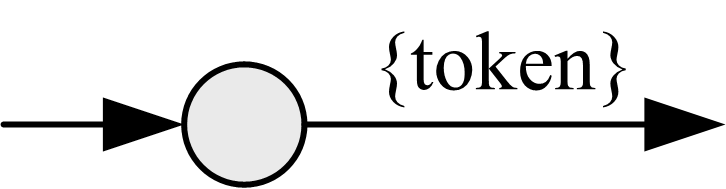
\includegraphics[scale=1.5]{pictures/auto_token}
  \caption{\label{fig:auto_token}Automāts vienam tokenam}
\end{figure}

Attēlā~\ref{fig:auto_sequence} ir parādīts NGA divu automātu konkatenācijai $e_1 e_2$.
\begin{figure}[H]
  \centering
    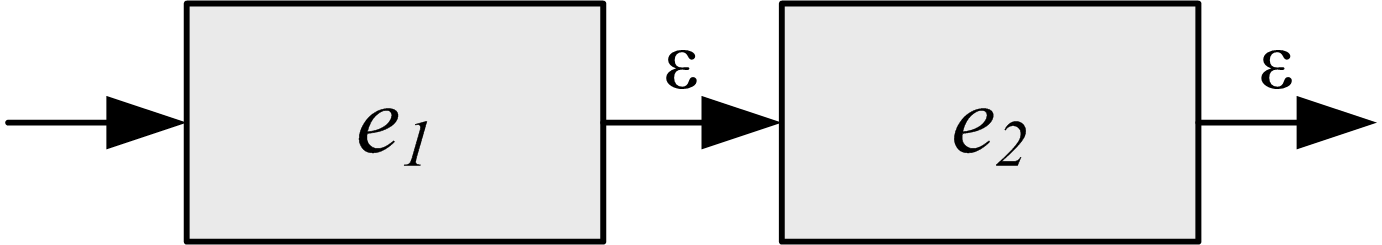
\includegraphics[scale=1.5]{pictures/auto_sequence}
  \caption{\label{fig:auto_sequence}Automāts divu automātu konkatenācijai}
\end{figure}

Attēlā~\ref{fig:auto_or} ir parādīts NGA izvēlei starp diviem automātiem $e_1 | e_2$.
\begin{figure}[H]
  \centering
    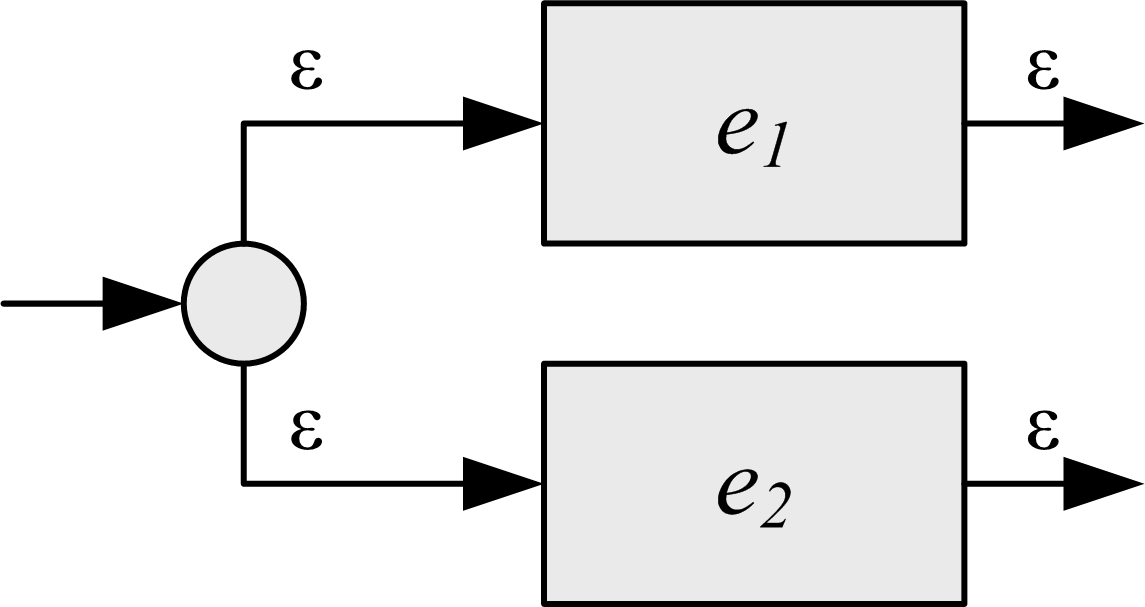
\includegraphics[scale=1.5]{pictures/auto_or}
  \caption{\label{fig:auto_or}Automāts izvēlei starp diviem automātiem}
\end{figure}

Attēlā~\ref{fig:auto_asterisk} ir parādīts NGA priekš konstrukcijas $e_1 *$.
\begin{figure}[H]
  \centering
    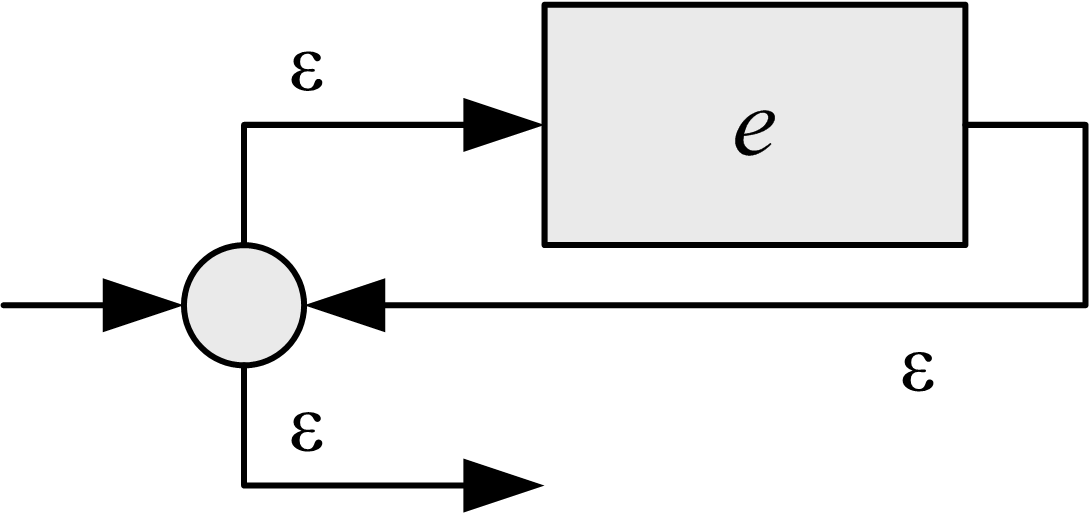
\includegraphics[scale=1.5]{pictures/auto_asterisk}
  \caption{\label{fig:auto_asterisk}Automats automātu virknei}
\end{figure}

Tālāk šie automāti tiek apvienoti vienā, un beigās tiek pievienots akceptējošais stāvoklis.

Apskatīsim piemēru - izteiksmi \verb/{id} ({real} | {int}) */. Sākumā tiek izveidoti NGA izteiksmes daļām. Attēls~\ref{fig:auto_token_id} parāda NGA priekš \verb|{id}|. Attēls~\ref{fig:auto_or_ex} parāda NGA priekš daļas \verb/{real} | {int}/. Attēls~\ref{fig:auto_asterisk_ex} parāda NGA priekš \verb/({real} | {int}) */.

\begin{figure}[H]
  \centering
    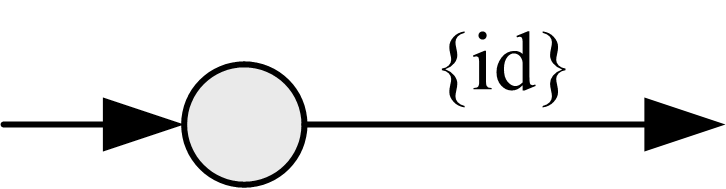
\includegraphics[scale=1.5]{pictures/auto_token_id}
  \caption{\label{fig:auto_token_id}Automats tokenam \texttt{\{id\}}}
\end{figure}

\begin{figure}[H]
  \centering
    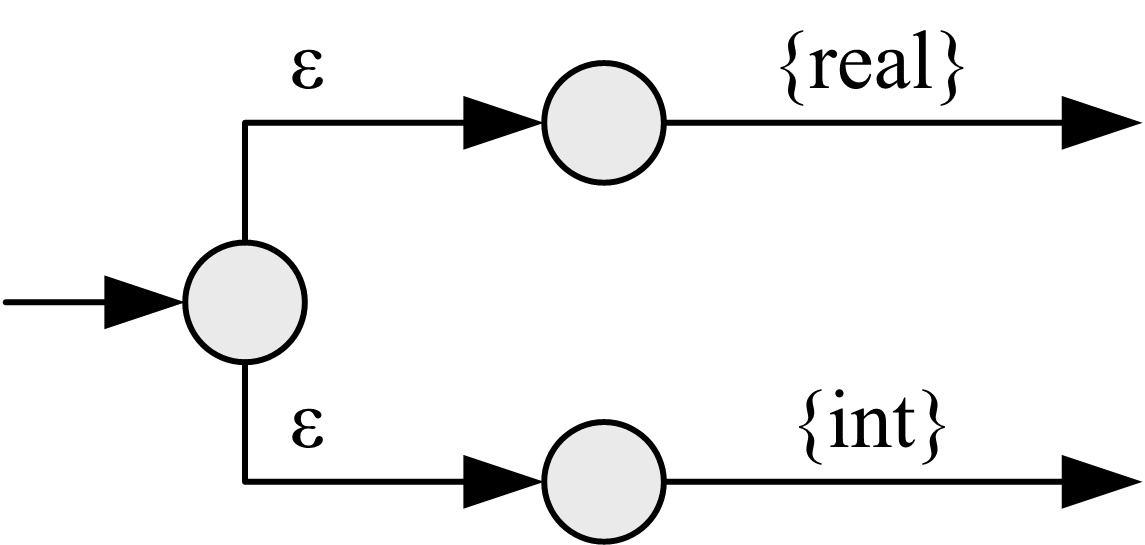
\includegraphics[scale=1.5]{pictures/auto_or_ex}
  \caption{\label{fig:auto_or_ex}Automats izteiksmei \texttt{\{real\} | \{int\}}}
\end{figure}

\begin{figure}[H]
  \centering
    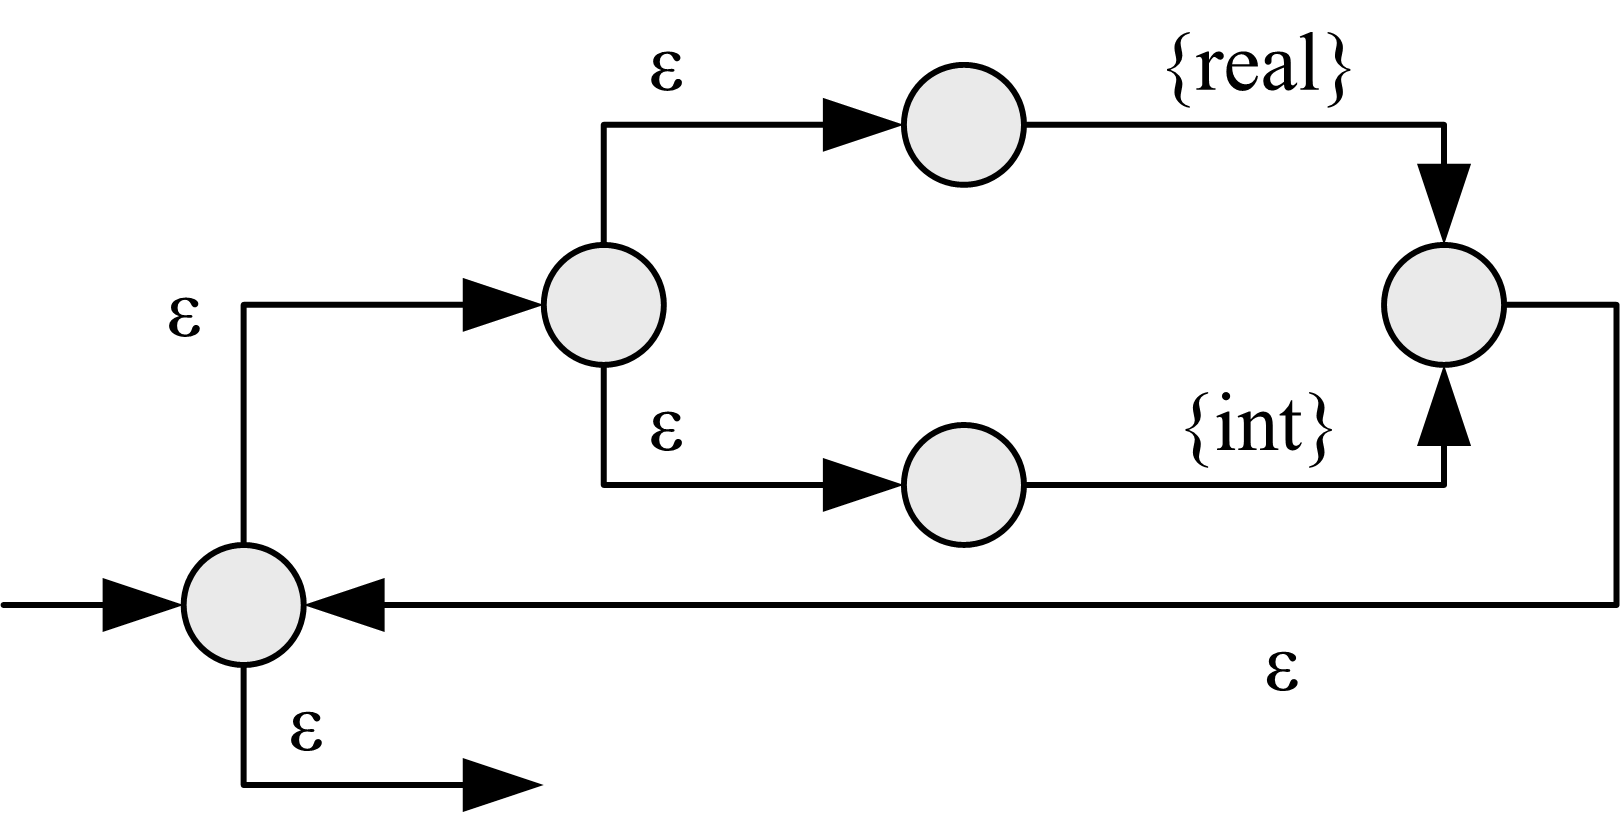
\includegraphics[scale=1.5]{pictures/auto_asterisk_ex}
  \caption{\label{fig:auto_asterisk_ex}Automats izteiksmei \texttt{(\{real\} | \{int\}) *}}
\end{figure}

Tad izveidotie automāti var tikt savienoti un beigās tiem tiek pievienots akceptējošais stāvoklis (attēls~\ref{fig:auto_full_ex}).

\begin{figure}[H]
  \centering
    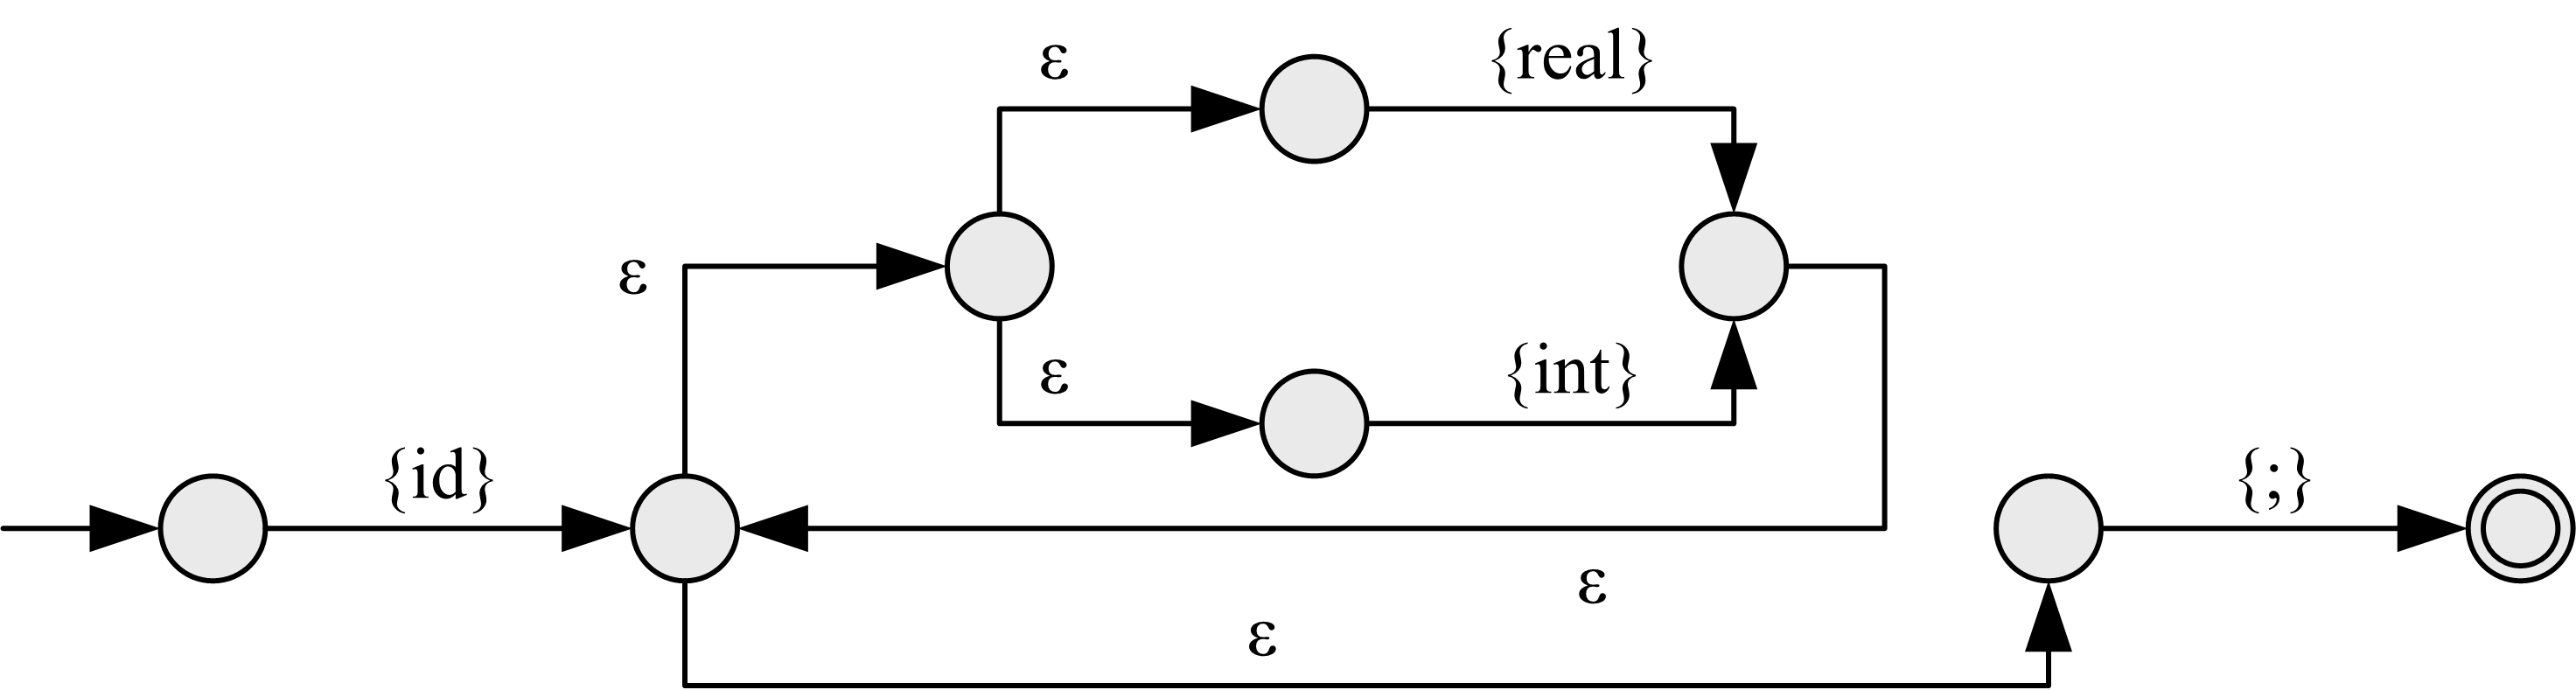
\includegraphics[scale=1.25]{pictures/auto_full_ex}
  \caption{\label{fig:auto_full_ex}Automats izteiksmei \texttt{\{id\} (\{real\} | \{int\}) *}}
\end{figure}

Tā tiek izveidots nedeterminēts automāts katrai regulārai izteiksmei. \cite{Cox:RegexpMatchingFast}, \cite{DragonBook}

\subsubsection{Determinizācija}

Kaut arī daudzām valodām ir vienkāršāk uzbūvēt nedeterminētu galīgu automātu (piemēram, pašām regulārām izteiksmēm tas ir loģiskāk), ir patiess tas, ka katra valoda var tikt aprakstīta gan ar nedeterminētu, gan ar determinētu galīgu automātu. Turklāt, dzīvē sastopamās situācijās DGA parasti satur tik pat daudz stāvokļu, cik ir NGA. Sliktākajā gadījumā, tomēr var gadīties, ka mazākais iespējamais DGA saturēs $m^n$ stāvokļu ($m$ - ieejas alfabēta elementu skaits), kamēr mazākais NGA saturēs $n$ stāvokļus. \footnote{Pieņemsim, ka automāta valoda sastāv no diviem simboliem - {0, 1}. Sliktākais gadījums, kad DGA tiešām saturēs $2^n$ stāvokļus attiecībā pret $n$ NGA stāvokļiem, var rasties tad, kad, piemēram, automāta valodā $n$-tais simbols no virknes beigām ir 1. Tad DGA būs jāprot atcerēties pēdējos $n$ simbolus. Tā kā ir divi ieejas alfabēta simboli, automātam ir jāatceras visas to dažādas $2^n$ kombinācijas.}

Izrādās, ka patiesībā katram NGA eksistē ekvivalents DGA, ko var uzbūvēt ar apakškopu sastādīšanas algoritmu \footnote{Pierādījumu tam, ka uzbūvētais DGA tik tiešām akceptē to pašu valodu, ko NGA, sk.  \cite{Hopcroft:IntroAutomataTheory}, teorēma 2.11.}. Vadošā doma šī algoritmā ir tas, ka katrs determinētā galīgā automāta (DGA) stāvoklis ir kādu NGA stāvokļu kopa. Pēc ieejas virknes $a_1, a_2, ..., a_n$ ielasīšanas DGA atrodas stāvoklī, kas atbilst NGA stāvokļu kopai, kuru var sasniegt apstaigājot virkni $a_1, a_2, ..., a_n$.

\paragraph*{Algoritms 1: NGA transformēšana uz DGA}
\subparagraph{Ieeja:}NGA $N$.
\subparagraph{Izeja:}DGA $D$, kas ir ekvivalents $N$.
\subparagraph{Algoritms:} Sākumā algoritms konstruē pāreju tabulu priekš $D$. Katrs $D$ stāvoklis ir $N$ stāvokļu kopa, tātad tabula tiek konstruēta tā, lai $D$ simulētu vienlaikus visas pārejas, ko var izpildīt $N$, saņemot kādu ieejas virkni. Lai automāts kļūtu determinēts, ir nepieciešams atbrīvoties no iespējas atrasties dažos stāvokļos vienlaikus. Tātad vajag atbrīvoties no $\varepsilon$-pārejām, un no daudzkārtīgām pārejām no viena stāvokļa pa vienu ieejas simbolu.

Tabulā~\ref{fig:NGAoperations} var redzēt divas funkcijas, kas ir nepieciešamas NGA apstrādes izpildei. Šīs funkcijas no NGA stāvokļiem un pārejām veido jaunas stāvokļu kopas, kuras veidos DGA stāvokļus.

\begin{table}[htdp]
  \caption{NGA apstaigāšanas funkcijas}
  \centering
  \begin{tabular}{|c|p{350pt}|}
    \hline
    Funkcija & Apraksts \\ \hline
    $\varepsilon-closure (T)$ & 
    NGA stāvokļu kopa, kas ir sasniedzama lietojot tikai $\varepsilon$-pārejas no visiem stāvokļiem no kopas $T$. \\ \hline
    $move (T, a)$ & 
    NGA stāvokļu kopa, kas ir sasniedzama lietojot pārejas pa simbolu $a$ no visiem stāvokļiem no kopas $T$. \\
    \hline
  \end{tabular}
\label{fig:NGAoperations}
\end{table}

Ir nepieciešams apstrādāt visas tādas $N$ stāvokļu kopas, kuras ir sasniedzamas, $N$ saņemot kaut kādu ieejas virkni. Indukcijas bāzes pieņēmums ir tas, ka pirms darbības uzsākšanas $N$ var atrasties jebkurā no stāvokļiem, kurus var sasniegt pārejot pa $\varepsilon$ bultiņām no $N$ sākuma stāvokļa. Ja $s_0$ ir $N$ sākuma stāvoklis, $D$ sākuma stāvoklis būs $\varepsilon-closure (set (s_0))$. Indukcijai pieņemam, ka $N$ var atrasties $T$ stāvokļu kopā pēc virknes $x$ ielasīšanas. Tad, ja $N$ ielasīs nākamo simbolu $a$, tad $N$ var pārvietoties jebkura no stāvokļiem $move (T, a)$. Taču pēc $a$ ielasīšanas var notikt vēl dažas $\varepsilon$-pārejas, tāpēc pēc virknes $xa$ ielasīšanas $N$ var atrasties jebkurā no stāvokļiem $\varepsilon-closure (move (T, a))$. Attēls~\ref{fig:det_algorithm} parāda pseido-kodu algoritmam, kā šādā veidā var tikt uzkonstruēti visi DGA stāvokļi un tā pāreju tabula.

Automāta $D$ sākuma stāvoklis ir $\varepsilon-closure (set (s_0))$, bet $D$ akceptējošie stāvokļi ir visas tās NGA stāvokļu kopas, kas satur vismaz vienu akceptējošu stāvokli. $Dstates$ ir jauna automāta $D$ stāvokļu saraksts un $Dtran$ ir stāvokļu pāreju tabula.

\begin{figure}[h]
  \begin{algorithmic}
  \State initially, $\varepsilon-closure (set (s_0))$  is the only state in $Dstates$, and is unmarked
  \While{there is an unmarked state $S$ in $Dstates$}
      \State mark $S$
      \For{each available oath $t$ from $S$} 
          \State $U = \varepsilon-closure (move (S, a))$
          \If {$U$ is not in $Dstates$}
              \State add $U$ as an unmarked state to $Dstates$
          \EndIf
          \State $Dtran [S, a] = U$;
      \EndFor
  \EndWhile
  \end{algorithmic}
  \caption{\label{fig:det_algorithm}Automāta determinizēšanas algoritms}
\end{figure}

\subparagraph{Sarežģītība:} Sarežģītības novērtējums šīm algoritmam ir diezgan nepatīkams. Sliktākajā gadījumā tas būs $O(m^(n+1))$, kur $n$ ir NGA stāvokļu daudzums un $m$ ir ieejas alfabēta simbolu skaits. Algoritms var uzģenerēt līdz $m^n$ DGA stāvokļiem, katram no kuram ir $m$ pārejas. Taču parasti tas tā nenotiek un DGA stāvokļu skaits ir līdzīgs NGA stāvokļu skaitam, un algoritma sarežģītība ir $O(n*m)$. \cite{DragonBook, Hopcroft:IntroAutomataTheory}

\subsubsection{\label{sbsbs:sol_minimization}Minimizēšana}

Izveidotais determinēts galīgs automāts var būt neoptimāls pēc stāvokļu skaita. Bet no šī skaitļa ir atkarīgs tālāko soļu izpildes ātrums. Tātad ir nepieciešams izveidot automātu, kas atpazīs to pašu valodu un saturēs minimālu iespējamu stāvokļi skaitu.

Var pierādīt, ka katram automātam eksistē ekvivalents minimāls automāts \footnote{Šī fakta pierādījumu sk. ???}. Vēl vairāk, ja eksistē 2 dažādi automāti ar vienādu stāvokļu daudzumu, kas atpazīst vienu un to pašu valodu, tad tie ir vienādi līdz stāvokļu nosaukumiem \footnote{Tā kā stāvokļu nosaukumi neietekmē automāta darbību, divi automāti tiek saukti par vienādiem līdz pat stāvokļu nosaukumiem, ja viens no tiem var tikt pārveidots otrajā vienkārši pārsaucot to stāvokļus.}.

Tālāk teiksim, ka virkne $x$ atšķir stāvokļu $s$ no stāvokļa $t$ tad, kad tikai viens stāvoklis, ko var sasniegt no $t$ un $s$ pa $x$ ir akceptējošs. Tātad divi stāvokļi ir atšķirami tad, kad eksistē tāda virkne, kas viņus atšķir. Jebkurš akceptējošs stāvoklis ir atšķirams no jebkura neakceptējoša stāvokļa ar tukšu virkni (stāvoklis nevar būt akceptējošs un neakceptējoss vienlaikus). Divi neatšķirami stāvokļi ir ekvivalenti. \footnote{\cite{Hopcroft:IntroAutomataTheory} nodaļa 4.4}

\paragraph*{Algoritms 2: DGA minimizēšana}
\subparagraph{Ieeja:}DGA $D$.
\subparagraph{Izeja:}Jauns DGA $D'$, kas ir minimāls un ekvivalents $D$.
\subparagraph{Algoritms:} 

Minimizēšanas algoritma vadošā doma ir sadalīt automātu neatšķiramos stāvokļu grupās. Tas izveido ekvivalentu stāvokļu grupas, kas tālāk var tikt apvienotas vienā, izveidojot minimāla automāta stāvokļus.

Minimizēšanas gaitā automāta stāvokļi tiek sadalīti grupās, ko uz doto brīdi algoritms nevar atšķirt. Jebkuri divi stāvokļi no dažādām grupām ir atšķirami. Katrā nākamajā algoritma iterācijā eksistējošās grupas tiek sadalītas mazākajās grupās, gadījumā, ja kādā grupā parādās atšķirami stāvokļi. Algoritms apstājas līdz ko neviena grupa nevar tikt sadalīta sīkāk.

Pirms algoritms uzsāk darbu, stāvokļi tiek sadalīti divās grupās - akceptējošie stāvokļi un neakceptējošie stāvokļi. Šo grupu stāvokļi ir atšķirami ar tukšu virkni. Tālāk tiek pa vienai apstrādātas grupas no pašreizējā sadalījums. Katrai grupai tiek pārbaudīts, vai tās stāvokļi var tikt atšķirti ar kādu ieejas simbolu - vai kāds no ieejas simboliem noved uz divām vai vairākām dažādam stāvokļu grupām. Ja tādi simboli eksistē, tiek izveidotas jaunas grupas, tādas, ka divi stāvokļi atrodas vienā grupā tad un tikai tad, ja tie aiziet uz vienādām grupām pa vienādiem simboliem. Process ir atkārtots visām pašreizējā sadalījuma grupām, tad atkal jaunam sadalījumam, kamēr neviena no grupām vairs nevar tikt sadalīta.

Attēls~\ref{fig:min_algorithm} parāda minimizēšanas algoritmu pseido-kodā.

\begin{figure}[h]
  \begin{algorithmic}
  \State initially, partitioning $\Pi$ contains two groups, $F$ and $S-F$, the accepting and nonaccepting states of $D$, $\Pi_{new}$ is empty
  \While{$\Pi_{new}$ is not equal to $\Pi$}
      \State $\Pi_{new} = \Pi$
      \For{each group $G$ of $\Pi$}
          \State partition $G$ into subgroups such that two states $s$ and $t$ are in the same subgroup if and only if for all input symbols $a$, states $s$ and $t$ have transitions on $a$ to states in the same group of $\Pi$
          \State replace $G$ in $\Pi_{new}$ by the set of all subgroups formed
      \EndFor
  \EndWhile
  \State $\Pi_{final} = \Pi$
  \end{algorithmic}
  \caption{\label{fig:min_algorithm}Automāta minimizēšanas algoritms}
\end{figure}

Tālāk paliek apstrādāt jaunizveidotās stāvokļu grupas izveidojot jaunu determinētu automātu. Lai to izdarītu, no katras sadalījuma $\Pi_{final}$ grupas tiek izvēlēts grupas pārstāvis. Grupu pārstāvji izveidos jaunus stāvokļus automātam $D'$. Pārējās komponentes minimālam automātam $D'$ tiks iveidotas sekojoši:
\begin{enumerate}
\item Automāta $D'$ sākuma stāvoklis ir pārstāvis tai grupai, kura satur automāta $D$ sākuma stāvokli.
\item Automāta $D'$ akceptējošie stāvokļi ir pārstāvji tām grupām, kuras satur automāta $D$ akceptējošos stāvokļus. Katra no grupām satur vai nu tikai akceptējošus, vai nu tikai neakceptējošus stāvokļus, jo algoritma darba gaitā jaunās grupas tika izveidotas tikai sadalot jau eksistējošas grupas, bet sākuma sadalījums atdalīja šīs stāvokļu klases.
\item Pieņemsim, ka $s$ ir kādas $\Pi_{final}$ grupas $G$ pārstāvis, un automāts $D$ no stāvokļa $s$ pa ieejas simbolu $a$ pāriet uz stāvokli $t$. Pieņemsim, ka $r$ ir grupas $H$ pārstāvis, $H$ satur $t$. Tad automātā $D'$ ir pāreja no stāvokļa $s$ uz stāvokli $r$ pa ieejas simbolu $a$.
\end{enumerate}

\subparagraph{Sarežģītība:}
Šī algoritma sarežģītība ir $O(n^2*l)$, kur $n$ ir sākotnējā automāta stāvokļu daudzums un $l$ maksimāls pāreju daudzums no kāda no stāvokļiem \footnote{Patiesībā $l$ būtu jābūt ieejas alfabēta elementu skaitam. Bet šī darba ietvaros ir atļauts veidot regulārās izteiksmes ar pārejām pa tokeniem ar specificētu vērtību, piemēram \texttt{\{int:5\}}. Tātad īstenībā ieejas alfabēts ir bezgalīgs.}.

\subsubsection{Apvienošana}

Kā jau bija teikts agrāk, lai samazinātu sakrišanu meklēšanas laiku, tika izvēlēts apvienot visus meklēšanas automātus vienā. Tā kā makro atnāk pa vienam dažādās vietās programmas kodā un var sākt uzreiz tikt lietotas, nav iespējams gaidīt kamēr sakrāsies vairāki automāti apvienošanai. Tikko parādās divi automāti tie tūlīt pat tiek apvienoti vienā sistēmā. Tālāk, kad parādās citi makro, to automāti tiek pievienoti jau eksistējošam.

Algoritms pēc savas būtības ir ļoti līdzīgs determinēšanas algoritmam. Vienīgais uzņēmums ir tas, ka nevienā no automātiem neeksistē $\varepsilon$-pārejas. Tātad tas, no kā vajag atbrīvoties, ir pārejas pa vienu un to pašu simbolu uz diviem dažādiem stāvokļiem. Tas tiek darīts apvienojot divus stāvokļus no dažādiem automātiem. 

\paragraph*{Algoritms 3: Divu DGA apvienošana}
\subparagraph{Ieeja:}DGA $D_1$ un $D_2$.
\subparagraph{Izeja:}Jauns DGA $D'$, kas apvieno $D_1$ un $D_2$.
\subparagraph{Algoritms:} 

Algoritms sāk darbu apvienojot $D_1$ un $D_2$ sākuma stāvokļus. Šo stāvokļu kombinācija veido automāta $D'$ sākuma stāvokli. Tālāk algoritms apskata visas iespējamas pārejas no katra no kombinētiem stāvokļiem un apvieno to rezultātus jaunajos stāvokļos. 

Apskatīsim piemēru automātu apvienošanai. Attēls~\ref{fig:auto_m_1} parāda determinētu minimālu automātu priekš regulārās izteiksmes \verb|{id}* {int}*|. Tas satur divus stāvokļus, \verb|a| un \verb|b|, kuri abi ir akceptējoši. Attēls~\ref{fig:auto_m_2}, savukārt, parāda DGA priekš izteiksmes \verb|{id} {real}* {int}|.

\begin{figure}[H]
  \centering
    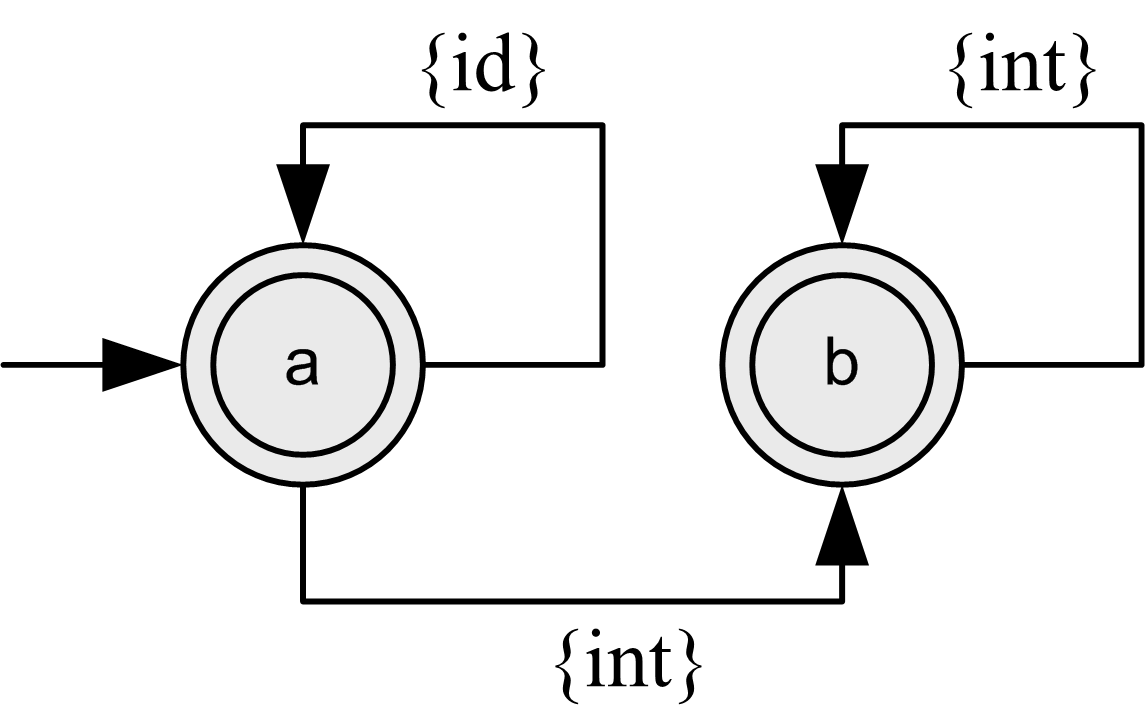
\includegraphics[scale=1.5]{pictures/auto_m_1}
  \caption{\label{fig:auto_m_1}Automats izteiksmei \texttt{\{id\} (\{real\} | \{int\}) *}}
\end{figure}

\begin{figure}[H]
  \centering
    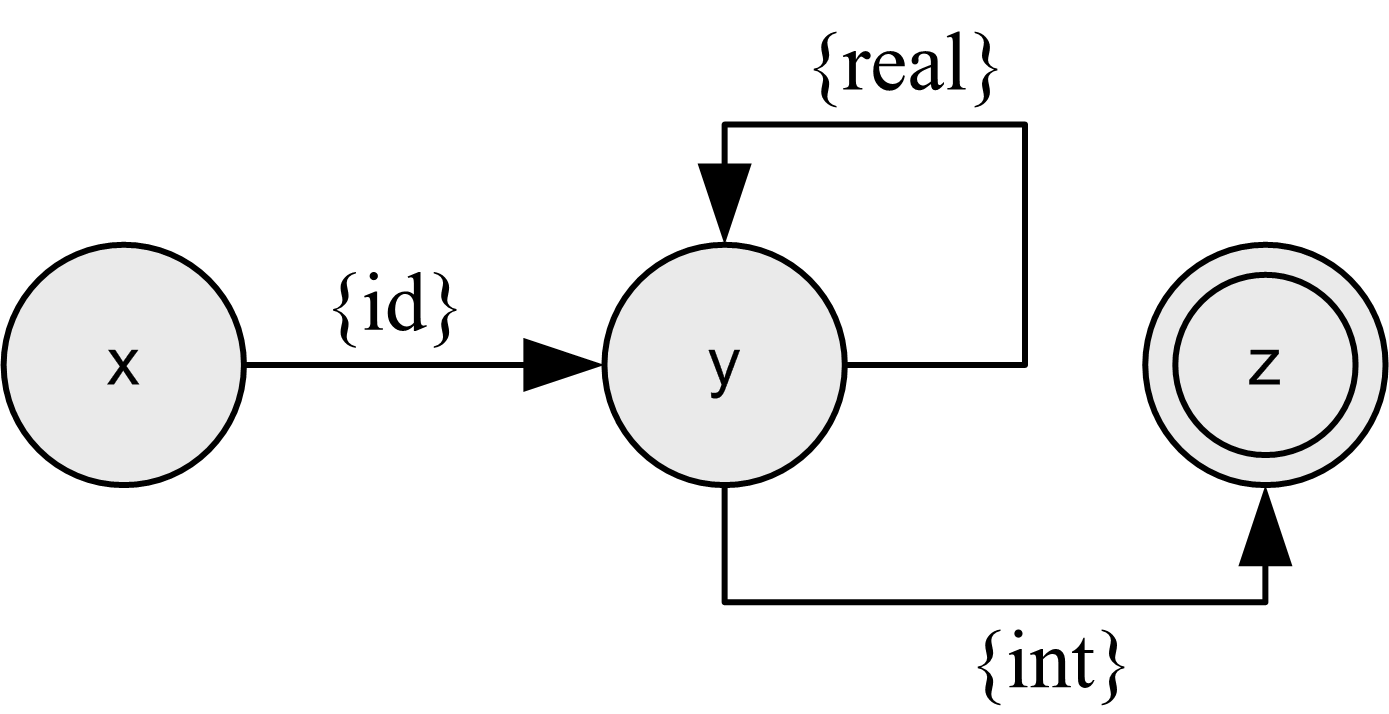
\includegraphics[scale=1.5]{pictures/auto_m_2}
  \caption{\label{fig:auto_m_2}Automats izteiksmei \texttt{\{id\} (\{real\} | \{int\}) *}}
\end{figure}

To apvienotais automāts ir parādīts attēlā~\ref{fig:auto_merge}.

\begin{figure}[H]
  \centering
    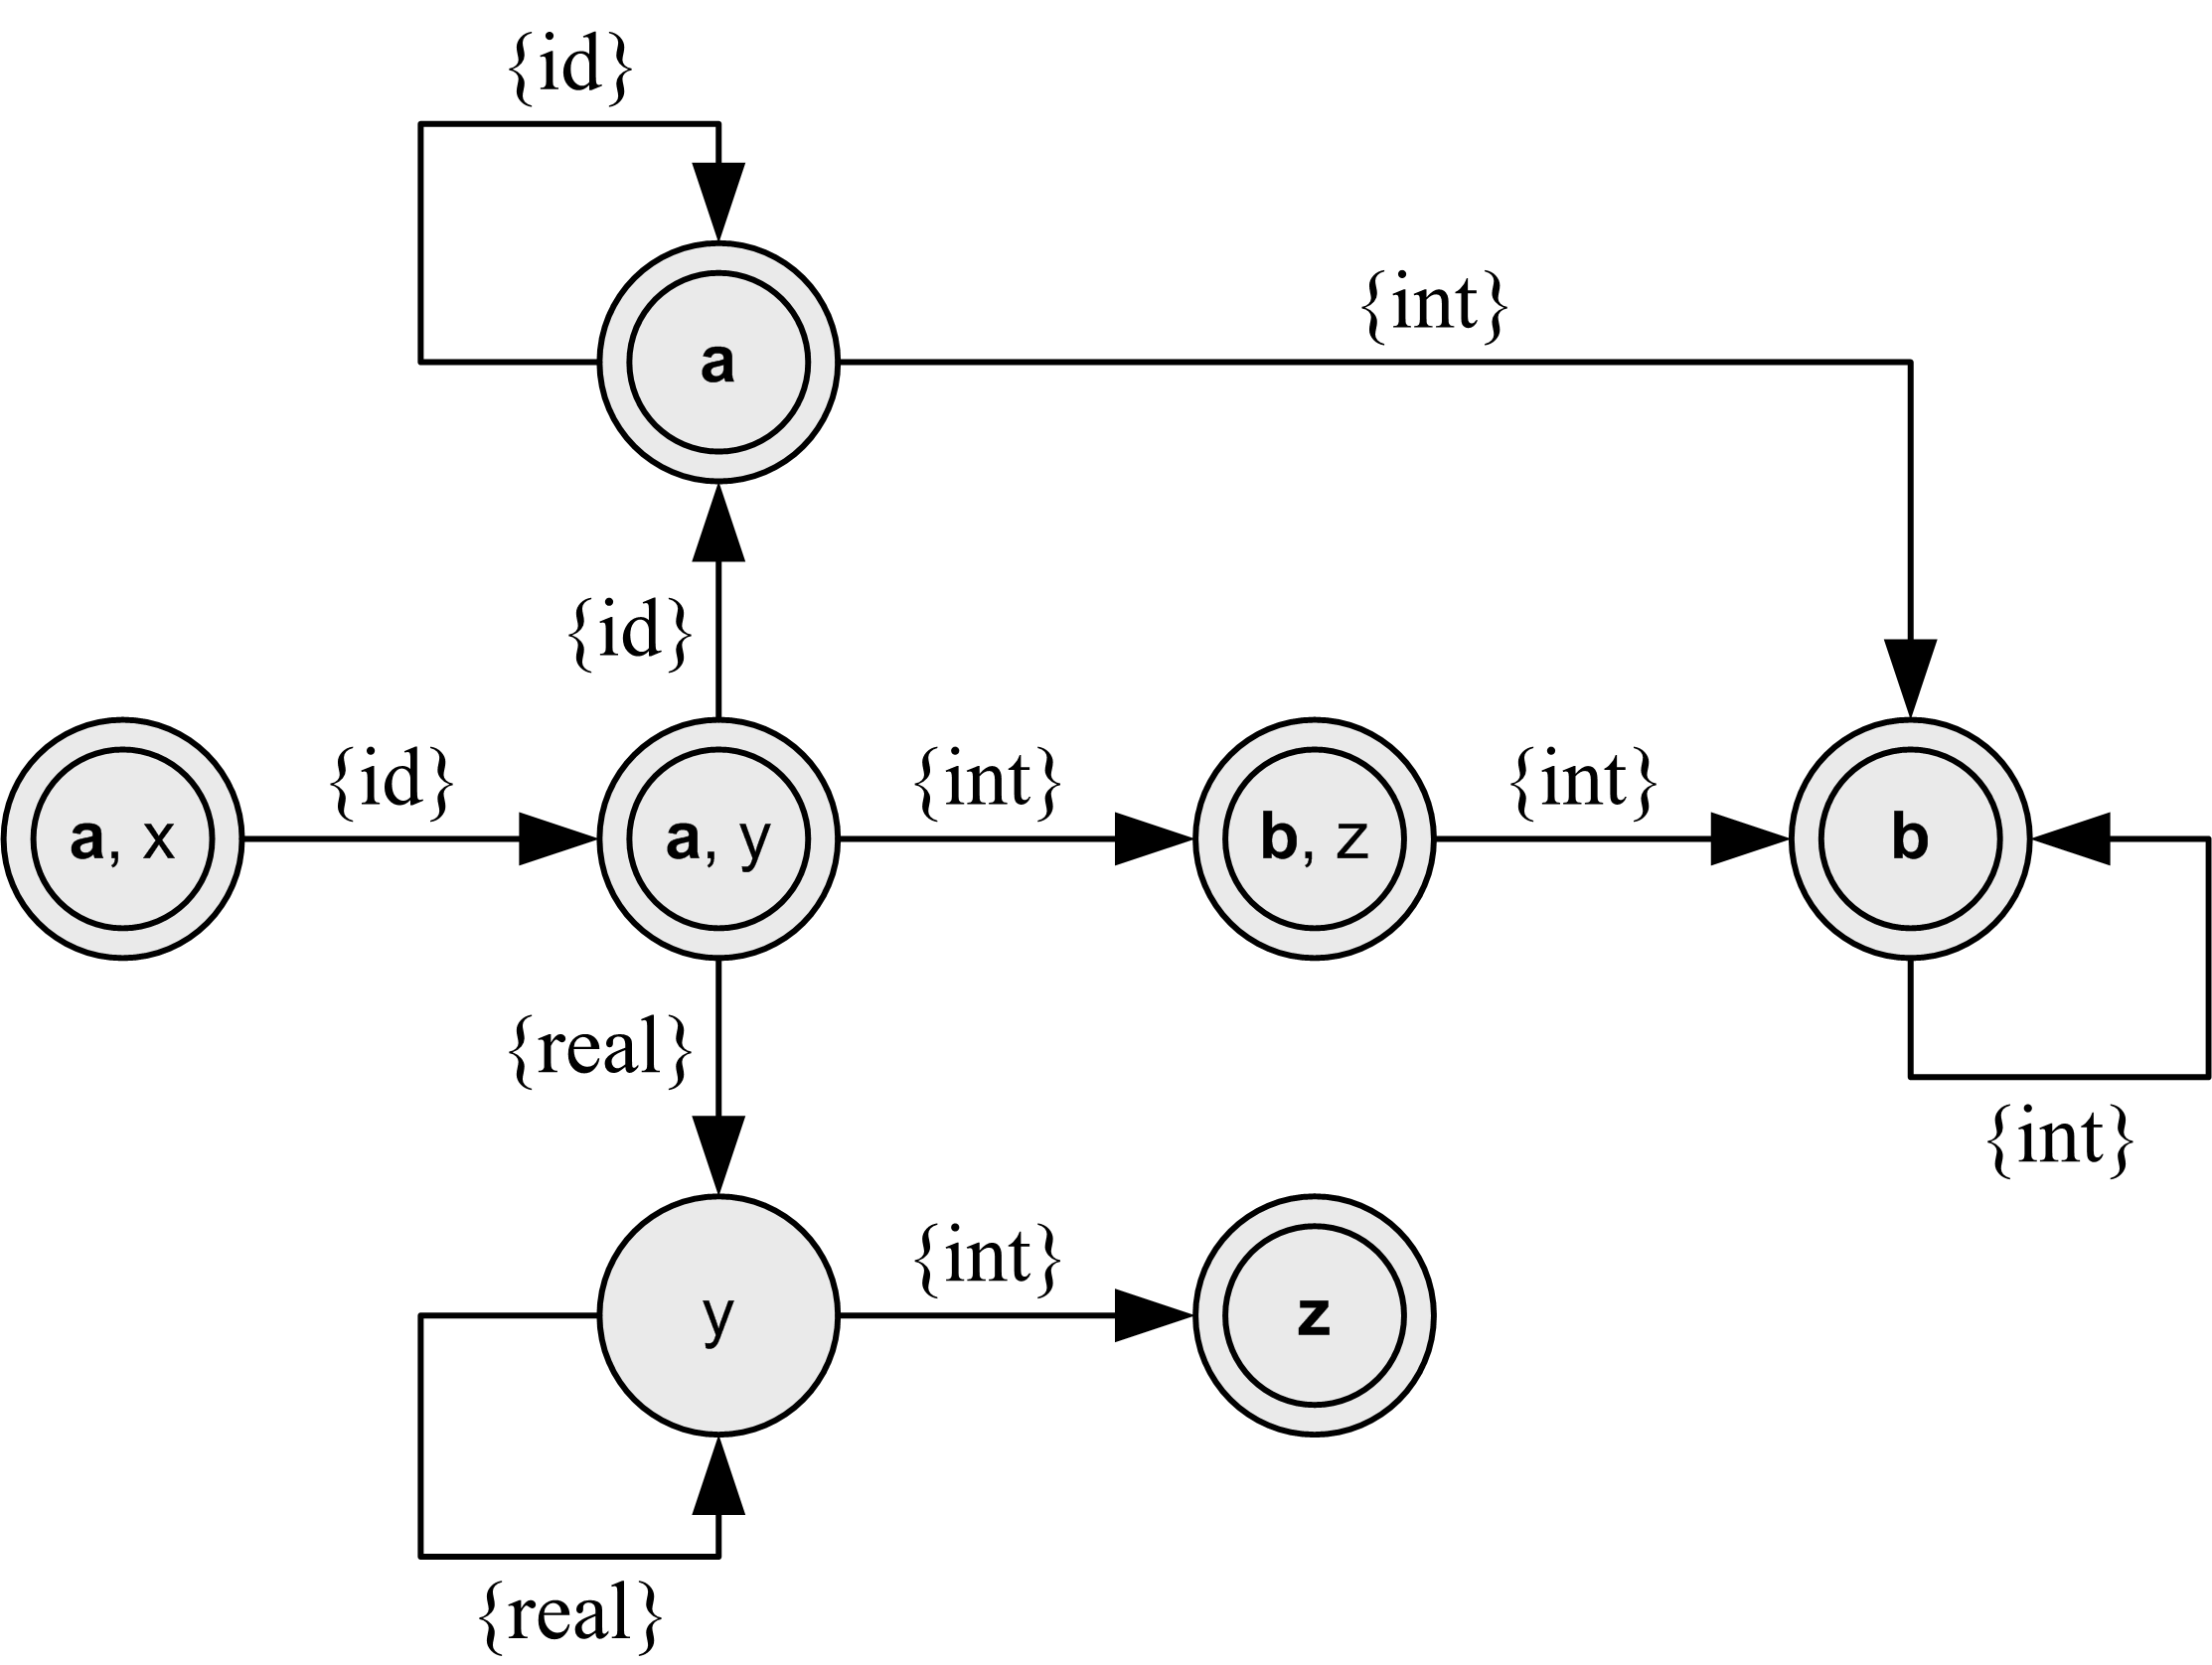
\includegraphics[scale=1.5]{pictures/auto_merge}
  \caption{\label{fig:auto_merge}Automats izteiksmei \texttt{\{id\} (\{real\} | \{int\}) *}}
\end{figure}

Attēls~\ref{fig:uni_algorithm} parāda apvienošanas algoritmu pseido-kodā. $s_0$ ir jaunā automāta $D'$ sākuma stāvoklis, $r_0$ ir $D_1$ sākuma stāvoklis un $t_0$ ir $D_2$ sākuma stāvoklis. $Dstates$ ir automāta $D'$ stāvokļu saraksts, $Dtran$ ir $D'$ pāreju tabula. Funkcija $move (S, t)$ atgriež tos stāvokļus, uz kuriem var nokļūt no $S$ pa tokenu $t$. Tā kā parasti $S$ sastāv no diviem stāvokļiem $r_i$ un $t_i$, tā atgriež pārejas rezultātu no katra no tiem. Rezultāts arī var but tikai viens stāvoklis, gadījumā, ja no kāda $r_i$ un $t_i$ neeksistē pāreja pa doto tokenu.

\begin{figure}[h]
  \begin{algorithmic}
  \State initially, $s_0 = (r_0, t_0)$ is the only state in $Dstates$, and is unmarked
  \While{there is an unmarked state $S$ in $Dstates$}
      \State mark $S$
      \For{each available move $t$ from $S$} \Comment{$S$ is a combination of some states $r_i$ and $t_i$ of $D_1$ and $D_2$, although it might be just a single state from one of the automata.}
          \State $U = move (S, t)$
          \If {$U$ is not in $Dstates$}
              \State add $U$ as an unmarked state to $Dstates$
          \EndIf
          \State $Dtran [S, t] = U$;
      \EndFor
  \EndWhile
  \end{algorithmic}
  \caption{\label{fig:uni_algorithm}Divu automātu apvienošanas algoritms}
\end{figure}

\subparagraph{Sarežģītība:}
Šī algoritma sarežģītība ir $O(n*m*l)$, kur  $n$ ir pirmā automāta stāvokļu daudzums, $m$ ir otrā automāta stāvokļu daudzums, un $l$ maksimāls pāreju daudzums no katra no stāvokļiem.

\subsubsection{Sakrišanu meklēšana}
Sakrišanu meklēšana NGA sliktākajā gadījumā būs ar sarežģītību $O(n^2*l)$, kur $n$ ir NGA stāvokļu skaits un $l$ - pārbaudāmās virknes elementu skaits. Tas var notikt, kad visi NGA stāvokļi ir aktīvi vienā laika brīdī, un no katra no tiem eksistē $n$ pārejas pa ieejas simbolu uz visiem automāta stāvokļiem.

Tīrā DGA gadījumā sakrišanu pārbaude katram ieejas elementam ir $O(l)$, kur $l$ ir pārbaudāmās virknes garums. 

Diemžēl pilnībā lineāra laika sakrišanu meklēšana nav iespējama tādēļ, ka prototips dod iespēju lietot makro ar tokenu vērtībām. Piemēram, eksistē 2 makro, viens no kuriem gaida tokenu \verb|{id}|, un otrs \verb|{id:foo}|. Gadījumā, kad sakrišanu meklēšanas procesā parādās tokens \verb|{id:foo}|, automātam nav iespējas izsecināt, kurš no ceļiem novedīs pie garākas sakritības. Tādēļ tas iet pa abiem ceļiem vienlaikus, saglabājot abus stāvokļus.

Kaut arī tas ievieš nedeterminētību, tā var parādīties tikai augstāk minētā gadījumā un izveidot ne vairāk ka 2 ceļus vienlaikus. Tātad kaut arī nedeterminētība pastāv, tai ir ļoti maza iespējamība un maza ietekme uz sakrišanu meklēšanas laiku.

\subsubsection{Tvērumi}

Viena no galvenām šīs sistēmas īpašībām ir iespēja atšķirt programmatūras tvērumus. Ir dažādi veidi, kā var izveidot automātus, kas atšķirtu atsevišķu tvērumu makro. Viens no veidiem varētu būt tāds - katram tvērumam izveidot automātu rindu, kur tvērumam specifiskākie automāti tiks pārbaudīti pirmie. Bet gadījumā, ja ir $n$ iekļautie tvērumi un nepieciešamais makro ir atrodams pirmajā automātā, būs jāizpilda vismaz $n$ meklēšanas, līdz ko pareizais šablons tiks atrasts. Atstājot tikai vienu aktīvu automātu vienā laika brīdī, arī ir dažas iespējas. Varētu visus šablonus likt vienā automātā kopā, un tad pēc izejas no tvēruma attiecīgos šablonus dzēst ārā. Tas nozīmētu, ka katram tvērumam jāatceras makro, kas tika pievienoti, un jāprot dzēst daļu no stāvokļiem ārā no automāta. Bet stāvokļu dzēšana ir laikietilpīga operācija, jo tās izpildīšanai būs nepieciešams apstaigāt visu lielo automātu, dzēšot no tā nevajadzīgos stāvokļus.

Tāpēc tika izvēlēta sekojoša pieeja. Ja prototips darba gaitā sastapās ar tvēruma sākuma simbolu, tas izveido eksistējošā automāta kopiju un ieliek to kaudzē. Tad automātam tiek pievienotas tvēruma makro. Izejot no tvēruma tā specifiskais automāts tiek izmests ārā un darbs tiek turpināts ar pēdējo automātu no kaudzes, kas atbilst iepriekšējam tvērumam. Šādā veidā jebkurā laika brīdī aktīvs ir tikai viens sakrišanu meklēšanas automāts.

\subsection{\label{sbs:sol_problems}Izņēmumi}

\subsubsection{Transformācijas}

Izstrādātais prototips nenodarbojas ar tokenu virkņu transformācijām, jo tā nav sakrišanu meklēšanas mehānisma uzdevums. Tālākajā sistēmas izstrādes gaitā notiks integrācija ar transformāciju sistēmu vai arī abu mehānismu sapludināšana vienā.

\subsubsection{Produkcijas}

Prototipā pagaidām nav implementēta apstrādes dalīšana pa gramatikas produkcijām, visas regulārās izteiksmes ir sapludinātas vienā automāta. Regulāro izteiksmju dalīšana pa tipiem tiks ieviesta vēlāk, kad tiks uzsākta integrācija un sadarbība ar reālu parsētāju. Tā varētu tikt implementēta līdzīgi tam, kā tiek realizēti konteksti - pa vienam sapludinātam automātam priekš katra produkcijas tipa.

\subsubsection{Tokenu klašu mantošana}

Sistēmai nav nekādas informācijas par valodas gramatiku. Tieši tāpēc tokens \verb|{real}| netiks uztverts ka \verb|{expr}|, kaut arī racionāls skaitlis ir izteiksme. Tā kā sistēmai jābūt neatkarīgai no valodas gramatikas, šī hierarhija nav iekodējama transformāciju sistēmā. To ir jānodrošina parsētājam, attiecīgi apstrādājot tokenus un apkopojot to nozīmi. Par to arī būs jārūpējas sistēmas lietotājam rakstot savas makro izteiksmes.

\subsubsection{Regulārās izteiksmes daļu grupēšana}

Tādēļ, ka aprakstītā pieeja mēģina pēc iespējas minimizēt meklēšanas laiku, tā neatļauj veidot atrasto tokenu grupēšanu, kā tas ir parasti pieņemts regulārās izteiksmēs. Tokenu grupēšana un atpakaļnorādes (\emph{backreferences}) uz tokenu grupām nav atļautas.

Tomēr ja parādīsies nepieciešamība, ir apskatīta arī pieeja, kas dos šādu iespēju. Tas varētu tikt izpildīts, determinējot tikai automāta stāvokļus grupu iekšienē, pēc tam ar $\varepsilon$-pārejām secīgi savienojot grupu automātu akceptējošus un sākuma stāvokļus. Automāts būs determinēts tikai grupu ietvaros, bet tad būs pieejamas atrasto tokenu grupas. Tomēr šāda pieeja neatļaus sapludināt dažus automātus vienā, jo sapludināšanas procedūra sabojās grupēšanu.

\subsubsection{Sapludinātā automāta minimizācija}

Automātu minimizēšana ir diezgan darbietilpīga operācija, tāpēc tā tiek izpildīta tikai uz atsevišķiem automātiem. Apvienotais visu šablonu automāts var nebūt minimāls, jo dažādu minimālu automātu apvienošana negarantē šo faktu. Bet tā kā apvienota automāta stāvokļu daudzums var būt ļoti liels, minimizēšanas izpilde var būt neefektīva. Tā kā minimizēšana samazina tikai automāta aizņemto vietu, nevis apstaigāšanas laiku, to šajā gadījumā var izlaist. Sapludinātā automāta minimizēšanu apgrūtina arī tas fakts, ka to stāvokļus vajadzēs atšķirt arī pēc tā fakta, kāds no šabloniem ir akceptēts, nevis tikai pēc tā, vai stāvoklis ir akceptējošs.

\subsection{\label{subsec:solution_optimization}Optimizācijas iespējas}

Regulāro izteiksmju optimizēšana uz doto brīdi netiek izpildīta, jo to ir vērts izpildīt uz regulārām izteiksmēm, kas tiks lietoti daudzas reizes. Darba apskatītā situācijā regulārās izteiksmes tiks lietotas tikai vienas programmas ietvaros un to optimizēšanai nav īpašas jēgas. Tomēr bez reāliem piemēriem nevar izšķirt, vai tas izveidos būtisku paātrinājumu šādā konkrētā gadījumā vai nē. Dažas regulāro izteiksmju pārrakstīšanas pieejas ir aprakstītas \cite{Yu:FMR}.

Dažreiz divu automātu sapludināšana var izraisīt pārāk lielu stāvokļu daudzumu rašanos. Ja reālajā situācijā tas ietekmēs apstrādes laiku, vai parādīsies nepieciešamība ierobežot automāta aizņemto laiku, var apskatīt iespēju glabāt dažus automātus viena vietā. \cite{Yu:FMR}

Minimizēšanas algoritmu var aizvietot ar citu, ātrāku algoritmu, piemēram, Hopkrofta minimizēšanas algoritmu, kura izpildes laiks ir $O(n$ log $n$ $l)$, kur $n$ ir automāta stāvokļu daudzums un $l$ ir ieejas alfabēta elementu daudzums.\cite{Berstel:MA}